\documentclass{article}
\usepackage{graphicx} % Required for inserting images
\usepackage{amsmath}
\usepackage[english, russian] {babel}
\usepackage[utf8]{inputenc}
\usepackage[T2A]{fontenc}
\usepackage{minted}
\usepackage{float}
\usepackage{amssymb}

\title{Теория графов}
\author{silvia.lesnaia }


\begin{document}

\maketitle

\textbf{19.19.25}

\section{Графы знаний}

Представление знаний - направление в исследованиях ИИ, посвященное
представлению информации о мире в форме, которую было бы возможно
использовать в компьютерных\dots

Социальные графы 

Молекулярные графы 

Графы знаний


Задачи на уровне  всего графа


Задачи на уровне вершин


Задачи на уровне ребер




уту много всего  надо запоннить 

\begin{figure} [H]
    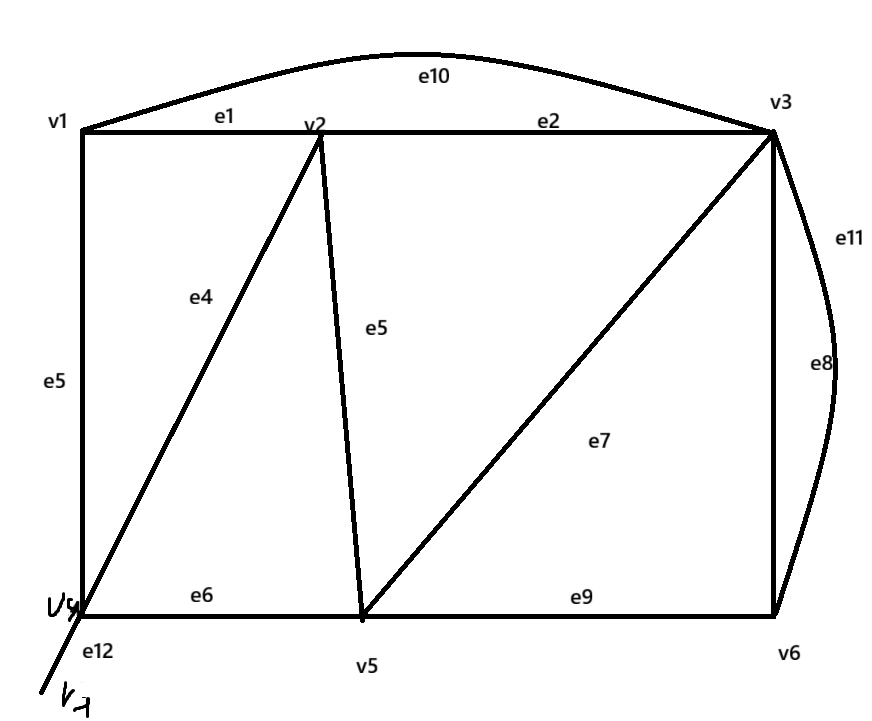
\includegraphics[width=0.50\linewidth]{Без имени.png}
\end{figure}

Маршурт

$V2\rightarrow V6$

$М1у10М3у11$





\dots




Расстояние d(x,y), между двумясвязаными вершинами x,y назвается длина наименьшого пути между нимми



\section{Алгоритм обходов}


\end{document}